%
% ---------------------------------------------------
%
% Trabajo Fin de Grado:
% Author: Víctor Hernández Pérez 
% Correo: alu0100697032@ull.edu.es
%
% ----------------------------------------------------
%
\documentclass[spanish,a4paper,14pt,oneside]{extreport}
%\documentclass[a4paper, twoside, 12pt]{book}
\usepackage[a4paper]{geometry}
\usepackage[spanish]{babel}
\usepackage[utf8]{inputenc}
%\usepackage{lscape}
\usepackage{pdflscape}
%%%%%%%%%%%%%%%%%%%%%%%%%%%%%%%%%%%%%%%%%%%%%%%%%%%%%%%%%%%%%%%%%%%%%%%%%%%%%%%%%%%%%%%%%%%%
% Next 3+3 lines select PDF or PS output (comment as apropriate)
% To switch from PDF and PS comment/uncomment here and change Makefile
\usepackage[pdftex]{color}
\usepackage[pdftex]{graphicx}
\graphicspath{{images/}}
%\usepackage[dvips]{color}
%\usepackage[dvips]{graphicx}
\usepackage{epsfig}
%\graphicspath{{images/eps/}} 
%%%%%%%%%%%%%%%%%%%%%%%%%%%%%%%%%%%%%%%%%%%%%%%%%%%%%%%%%%%%%%%%%%%%%%%%%%%%%%%%%%%%%%%%%%%%
\usepackage{algorithmic}
\usepackage[pdftex=true,colorlinks=false,urlcolor=blue,plainpages=false,pagebackref=true,citecolor=red]{hyperref} %hiperenlaces y backcites 
%%%%%%%%%%%%%%%%%%%%%%%%%%%%%%%%%%%%%%%%%%%%%%%%%%%%%%%%%%%%%%%%%%%%%%%%%%%%%%%%%%%%%%%%%%%%
% Comandos para escribir "siempre igual"
\newcommand{\App}{\texttt{ULL App{}}}

%%% Traducimos el pseudocodigo
\renewcommand{\algorithmicwhile}{\textbf{mientras}}
\renewcommand{\algorithmicend}{\textbf{fin}}
\renewcommand{\algorithmicdo}{\textbf{hacer}}
\renewcommand{\algorithmicif}{\textbf{si}}
\renewcommand{\algorithmicthen}{\textbf{entonces}}
\renewcommand{\algorithmicrepeat}{\textbf{repetir}}
\renewcommand{\algorithmicuntil}{\textbf{hasta que}}
\renewcommand{\algorithmicelse}{\textbf{en otro caso}}
\renewcommand{\algorithmicfor}{\textbf{para}}

%%%%%%%%%%%%%%%%% Creamos un entorno para listar código fuente %%%%%%%%%%%%%%%
\newenvironment{sourcecode}
{\begin{list}{}{\setlength{\leftmargin}{1em}}\item\scriptsize\bfseries}
{\end{list}}

\newenvironment{littlesourcecode}
{\begin{list}{}{\setlength{\leftmargin}{1em}}\item\tiny\bfseries}
{\end{list}}

\newenvironment{summary}
{\par\noindent\begin{center}\textbf{Abstract}\end{center}\begin{itshape}\par\noindent}
{\end{itshape}}

\newenvironment{keywords}
{\begin{list}{}{\setlength{\leftmargin}{1em}}\item[\hskip\labelsep \bfseries Keywords:]}
{\end{list}}

\newenvironment{palabrasClave}
{\begin{list}{}{\setlength{\leftmargin}{1em}}\item[\hskip\labelsep \bfseries Palabras clave:]}
{\end{list}}


%%%%%%%%%%%%%%%%%%%%%%%%%%%%%%%%%%%%%%%%%%%%%%%%%%%%%%%%%%%%%%%%%%%%%%%%%%%%%%%
\definecolor{marron}       {rgb}{0.496, 0.203, 0.152}
\definecolor{verde-claro}  {rgb}{0.625, 0.734, 0.199}
\definecolor{oscuro}       {rgb}{0.187, 0.141, 0.285}
\definecolor{gris}     	   {rgb}{0.500, 0.500, 0.500}
\definecolor{bgd-listings} {rgb}{0.999, 0.999, 0.900}
\definecolor{gray97}{gray}{.97}
\definecolor{gray75}{gray}{.75}
\definecolor{gray45}{gray}{.45}
\definecolor{gray}{gray}{.45}
%%%%%%%%%%%%%%%%%%%%%%%%%%%%%%%%%%%%%%%%%%%%%%%%%%%%%%%%%%%%%%%%%%%%%%%%%%%%%%%%%%%%%%%%%%%%
%%% Code Listings
%\usepackage{listings} 
%\lstloadlanguages{python,C}
\definecolor{Brown}{cmyk}{0,0.81,1,0.60}
\definecolor{OliveGreen}{cmyk}{0.64,0,0.95,0.40}
\definecolor{CadetBlue}{cmyk}{0.62,0.57,0.23,0}
\definecolor{lightlightgray}{gray}{0.9}
%%%%%%%%%%%%%%%%%%%%%%%%%%%%%%%%%%%%%%%%%%%%%%%%%%%%%%%%%%%%%%%%%%%%%%%%%%%%%%%%%%%%%%%%%%%
%Evitar partir palabras al final de la línea
%\hyphenpenalty=10000
%\tolerance=1000
%%%%%%%%%%%%%%%%%%%%%%%%%%%%%%%%%%%%%%%%%%%%%%%%%%%%%%%%%%%%%%%%%%%%%%%%%%%%%%%%%%%%%%%%%%%%
% Para listados de código
\usepackage{listings}
\lstloadlanguages{C}

% Definiendo colores para los listados de código fuente - Univ. Deusto
\definecolor{violet}{rgb}{0.5,0,0.5}
\definecolor{navy}{rgb}{0,0,0.5}
\definecolor{hellgelb}{rgb}{1,1,0.8}
\definecolor{colKeys}{rgb}{0,0,1}
\definecolor{colIdentifier}{rgb}{0,0,0}
\definecolor{colComments}{rgb}{1,0,0}
\definecolor{colString}{rgb}{0,0.5,0}

%\lstset{morekeywords={pragma copy\_in copy\_out copy omp parallel private reduction shared hicuda loop\_partition over\_tblock over\_thread}}
\lstset{
        float=tbhp,
		    language = Java,
				morekeywords={llc,reduction_type,nc_result,
				              hicuda,global,alloc,shape,kernel,thread,loop_partition,tblock,over_tblock,over_thread,kernel_end,copyout,free,
											data,region,
											task,input,inout,output,
				              pragma,omp,parallel,reduction,private,shared,target,device,copy_in,copy_out,
				              acc,kernels,loop,copyin,copy,pcopy,pcopyin,collapse,gang,worker,independent},
				%\emph      ={omp,parallel,reduction,private,shared},
				emphstyle=\textbf,
        %basicstyle=\ttfamily\tiny,
        basicstyle=\ttfamily\scriptsize,
        identifierstyle=\color{colIdentifier},
        keywordstyle=\color{colKeys},
        stringstyle=\color{colString},
        commentstyle=\color[rgb]{0.133,0.545,0.133},
        columns=flexible,
        tabsize=4,
        frame=single,
        extendedchars=true,
        showspaces=false,
        showstringspaces=false,
        numbers=left,
        numberstyle=\tiny,
        breaklines=true,
        backgroundcolor=\color{lightlightgray},
        breakautoindent=true,
        captionpos=b
}

%\renewcommand{\lstlistingname}{Listing} % Los títulos de los códigos insertados se denotan con Ejemplo...   

% Otro formato más bonito para código fuente
\newcommand{\codigofuente}[3]{%
  \lstlisting[language=#1,caption={#2}]{#3}%
}
%%%%%%%%%%%%%%%%%%%%%%%%%%%%%%%%%%%%%%%%%%%%%%%%%%%%%%%%%%%%%%%%%%%%%%%%%%%%%%%
\begin{document}
\renewcommand{\lstlistingname}{Listado}% Listing -> Listado de código
%%%%%%%%%%%%%%%%%%%%%%%%%%%%%%%%%%%%%%%%%%%%%%%%%%%%%%%%%%%%%%%%%%%%%%%%%%%%%%%
% First Page
%%%%%%%%%%%%%%%%%%%%%%%%%%%%%%%%%%%%%%%%%%%%%%%%%%%%%%%%%%%%%%%%%%%%%%%%%%%%%%%

\pagestyle{empty}
\thispagestyle{empty}


\newcommand{\HRule}{\rule{\linewidth}{1mm}}
\setlength{\parindent}{0mm}
\setlength{\parskip}{0mm}

\vspace*{\stretch{0.5}}

\begin{center}

\includegraphics[scale=0.8]{images/logo_vertical}\\[10mm]
{\Huge Trabajo de Fin de Grado}
\end{center}

\HRule
\begin{flushright}
        {\Huge Aplicación Android: \App{}} \\[2.5mm]
        %{\Large \textit{App} .} \\[5mm]
        {\Large Víctor Hernández Pérez} \\[5mm]


\end{flushright}
\HRule
\vspace*{\stretch{2}}
\begin{center}
  \Large La Laguna, \today
\end{center}

\setlength{\parindent}{5mm}

%%%%%%%%%%%%%%%%%%%%%%%%%%%%%%%%%%%%%%%%%%%%%%%%%%%%%%%%%%%%%%%%%%%%%%%%%%%%%%%
% Signature page (add the official stamp)
%%%%%%%%%%%%%%%%%%%%%%%%%%%%%%%%%%%%%%%%%%%%%%%%%%%%%%%%%%%%%%%%%%%%%%%%%%%%%%%
\newpage
%\cleardoublepage
\thispagestyle{empty}

D. {\bf Francisco de Sande González}, con N.I.F. 42.067.050-G
profesor
Titular de Universidad
adscrito al Departamento
de Ingeniería Informática y de Sistemas
de la Universidad de La Laguna, como tutor

\bigskip

\bigskip
\bigskip
{\bf C E R T I F I C A}

\bigskip
\bigskip
\bigskip
Que la presente memoria titulada:

\bigskip
``{\it \App{}}''

\bigskip
\bigskip
\bigskip

\noindent ha sido realizada bajo su dirección por D. {\bf Víctor Hernández Pérez},
con N.I.F. 78.643.409-S

\bigskip
\bigskip

Y para que así conste, en cumplimiento de la legislación vigente y a los efectos
oportunos firman la presente en La Laguna a \today

%\cleardoublepage
\newpage
%%%%%%%%%%%%%%%%%%%%%%%%%%%%%%%%%%%%%%%%%%%%%%%%%%%%%%%%%%%%%%%%%%%%%%%%%%%%%%%
\thispagestyle{empty}

{ \flushright

\begin{LARGE}
Agradecimientos
\end{LARGE}

\hspace{3mm}

\begin{large}


\hspace{3mm}
Agradezco ...


\end{large}

}

%%%%%%%%%%%%%%%%%%%%%%%%%%%%%%%%%%%%%%%%%%%%%%%%%%%%%%%%%%%%%%%%%%%%%%%%%%%%%%%%%
\newpage

\begin{huge}
Licencia
\end{huge}

\bigskip
%* Si quiere permitir que se compartan las adaptaciones de tu obra mientras se comparta de la misma manera
%y NO quieres permitir usos comerciales de tu obra indica:

\begin{center}

\includegraphics[scale=1.5]{images/by-nc-sa_88x31}\\[10mm]
{\Large \copyright~Esta obra está bajo una licencia de Creative Commons Reconocimiento-NoComercial-CompartirIgual 4.0 Internacional.
}
\end{center}


%%%%%%%%%%%%%%%%%%%%%%%%%%%%%%%%%%%%%%%%%%%%%%%%%%%%%%%%%%%%%%%%%%%%%%%%%%%%%%%
\newpage  %\cleardoublepage
\begin{abstract}
{\em

El objetivo de este trabajo ha sido crear una aplicación para dispositivos Android que permita ...

\bigskip
Partiendo de los conocimientos en \textit{Java} obtenidos en la asignatura: \textit{'Programación de Aplicaciones Interactivas'} y desarrollados en otras asignaturas como: 
\textit{'Diseño y Análisis de Algoritmos'}, \textit{'Complejidad Computacional'} o \textit{'Inteligencia Artificial'} impartidas, la mayor parte de las mismas, en el 
itinerario de computación del Grado en Ingeniería Informática de la Universidad de La Laguna, se espera adquirir los 
conocimientos básicos necesarios para desarrollar aplicaciones en Android. 

\bigskip
Del mismo modo... 

\bigskip 
También ...

}
\begin{palabrasClave}
Aplicaciones Android,.
\end{palabrasClave}

\end{abstract}
%%%%%%%%%%%%%%%%%%%%%%%%%%%%%%%%%%%%%%%%%%%%%%%%%%%%%%%%%%%%%%%%%%%%%%%%%%%%%%%

%%%%%%%%%%%%%%%%%%%%%%%%%%%%%%%%%%%%%%%%%%%%%%%%%%%%%%%%%%%%%%%%%%%%%%%%%%%%%%%
\newpage  %\cleardoublepage
\begin{summary}
{\em

The aim of this work has been the development of an application for Android devices that allows to ...

\bigskip
Based on the knowledge of Java obtained in the subject: ``Programming Interactive Applications'' and developed in other subjects like: ``Design and Analysis of Algorithms'', 
``Computational Complexity'' or``Artificial Intelligence''  taken, most of them, in the
Computer itinerary in the third year of the Universidad de La Laguna Degree in Computing Engineering, 
in this work we expect to acquire the basic knowledge needed to
develop Android applications.

\bigskip
Moreover ...

\bigskip
Finally ...

}

\begin{keywords}
Application for Android.
\end{keywords}

\end{summary}
%%%%%%%%%%%%%%%%%%%%%%%%%%%%%%%%%%%%%%%%%%%%%%%%%%%%%%%%%%%%%%%%%%%%%%%%%%%%%%%

%%%%%%%%%%%%%%%%%%%%%%%%%%%%%%%%%%%%%%%%%%%%%%%%%%%%%%%%%%%%%%%%%%%%%%%%%%%%%%%
\newpage{\pagestyle{empty}}
\thispagestyle{empty}

%%%%%%%%%%%%%%%%%%%%%%%%%%%%%%%%%%%%%%%%%%%%%%%%%%%%%%%%%%%%%%%%%%%%%%%%%%%%%%%


\pagestyle{myheadings} %my head defined by markboth or markright
% No funciona bien \markboth sin "twoside" en \documentclass, pero al
% ponerlo se dan un montón de errores de underfull \vbox, con lo que no se
% ha puesto.
\markboth{Víctor Hernández Pérez}{nombreApp}

%%%%%%%%%%%%%%%%%%%%%%%%%%%%%%%%%%%%%%%%%%%%%%%%%%%%%%%%%%%%%%%%%%%%%%%%%%%%%%%
%Numeracion en romanos
\renewcommand{\thepage}{\roman{page}}
\setcounter{page}{1}

%%%%%%%%%%%%%%%%%%%%%%%%%%%%%%%%%%%%%%%%%%%%%%%%%%%%%%%%%%%%%%%%%%%%%%%%%%%%%%%

\tableofcontents

%%%%%%%%%%%%%%%%%%%%%%%%%%%%%%%%%%%%%%%%%%%%%%%%%%%%%%%%%%%%%%%%%%%%%%%%%%%%%%%
\newpage{\pagestyle{empty}}

\listoffigures

%%%%%%%%%%%%%%%%%%%%%%%%%%%%%%%%%%%%%%%%%%%%%%%%%%%%%%%%%%%%%%%%%%%%%%%%%%%%%%%
\newpage{\pagestyle{empty}}

%\listoftables

%%%%%%%%%%%%%%%%%%%%%%%%%%%%%%%%%%%%%%%%%%%%%%%%%%%%%%%%%%%%%%%%%%%%%%%%%%%%%%%
\newpage{\pagestyle{empty}}

%%%%%%%%%%%%%%%%%%%%%%%%%%%%%%%%%%%%%%%%%%%%%%%%%%%%%%%%%%%%%%%%%%%%%%%%%%%%%%%
%Numeracion a partir del capitulo I
\renewcommand{\thepage}{\arabic{page}}
\setcounter{page}{1}


%%%%%%%%%%%%%%%%%%%%%%%%%%%%%%%%%%%%%%%%%%%%%%%%%%%%%%%%%%%%%%%%%%%%%%%%%%%%%%%
%\chapter{Introducción}
%\label{chapter:intro}
%\input{cap1.tex}
%%%%%%%%%%%%%%%%%%%%%%%%%%%%%%%%%%%%%%%%%%%%%%%%%%%%%%%%%%%%%%%%%%%%%%%%%%%%%%%
%\chapter{Título del Capítulo Dos}
%\label{chapter:dos}
%\input{cap2.tex}
%%%%%%%%%%%%%%%%%%%%%%%%%%%%%%%%%%%%%%%%%%%%%%%%%%%%%%%%%%%%%%%%%%%%%%%%%%%%%%%%
%\newpage{\pagestyle{empty}}
%\thispagestyle{empty}
%\chapter{Título del Capítulo Tres}
%\label{chapter:tres}
%\input{cap3.tex}
%%%%%%%%%%%%%%%%%%%%%%%%%%%%%%%%%%%%%%%%%%%%%%%%%%%%%%%%%%%%%%%%%%%%%%%%%%%%%%%%
%\chapter{Título del Capítulo Cuatro}
%\label{chapter:cuatro}
%\input{cap4.tex}
%%%%%%%%%%%%%%%%%%%%%%%%%%%%%%%%%%%%%%%%%%%%%%%%%%%%%%%%%%%%%%%%%%%%%%%%%%%%%%%%
%\newpage{\pagestyle{empty}}
%\thispagestyle{empty}
%\chapter{Conclusiones y líneas futuras}
%\label{chapter:Conclusiones}
%\input{cap5.tex}
%%%%%%%%%%%%%%%%%%%%%%%%%%%%%%%%%%%%%%%%%%%%%%%%%%%%%%%%%%%%%%%%%%%%%%%%%%%%%%%%
%\newpage{\pagestyle{empty}}
%\thispagestyle{empty}
%\chapter{Summary and Conclusions }
%\label{chapter:ingles}
%\input{cap6.tex}
% ==========================================================
% --------               Capítulos                ----------
% --------    Estan en el directorio capitulos/   ----------
% ==========================================================
%
% ---------------------------------------------------
%
% Trabajo Fin de Grado:
% Author: Víctor Hernández Pérez 
% Correo: alu0100697032@ull.edu.es
% Capítulo: Prólogo
%
% ----------------------------------------------------
%
\chapter*{Introducción}
\addcontentsline{toc}{chapter}{Introducción} 

En este documento se recoge el trabajo de investigación y desarrollo realizado por el 
autor para completar su Trabajo de Fin de Grado (TFG), finalizando con el mismo
los estudios en el Grado en Ingeniería en Informática cursados en la Escuela Superior 
de Ingerniería y Tecnología - Sección Informática (ESIT-Informática) de la ULL.


%
% ---------------------------------------------------
%
% Trabajo Fin de Grado:
% Author: Víctor Hernández Pérez 
% Correo: alu0100697032@ull.edu.es
% Capítulo: Objetivos
%
% ----------------------------------------------------
%

\chapter{Objetivos} \label{chap:objetives}  

El presente TFG ...

\begin{itemize}
\item Adquirir conocimientos básicos sobre conceptos, modelos, técnicas y herramientas asociadas con la programación de aplicaciones en Android.
\item Puesta en práctica de los conocimientos del Grado en Ingeniería Informática.
\item Creación de una memoria técnica sobre la aplicación desarrollada en el Trabajo de Fin de Grado.
\item Adquirir conocimientos sobre \textit{LaTeX} \cite{URL::LaTeX}, un sistema de composición de textos, orientado a la creación de documentos escritos 
que presenten una alta calidad tipográfica.
\end{itemize}

%
% ---------------------------------------------------
%
% Trabajo Fin de Grado:
% Author: Víctor Hernández Pérez 
% Correo: alu0100697032@ull.edu.es
% Capítulo: Herramientas Software
%
% ----------------------------------------------------
%

\cleardoublepage
\chapter{Herramientas y Tecnologías Software} \label{chap:polytopes}  

En este capítulo se describen las herramientas y tecnologías que han sido usadas para la 
elaboración del trabajo, tanto la aplicación móvil como la memoria.

\section{Herramientas}
En esta sección se explicarán las herramientas de trabajo utilizadas.
\subsection{Android Studio}

Android Studio \cite{URL::AndroidStudio} es un nuevo entorno de desarrollo 
integrado para el sistema operativo Android comercializado por Google, 
diseñado para ofrecer nuevas herramientas para el desarrollo de aplicaciones y 
alternativa al entorno Eclipse \cite{URL::Eclipse}, 
hasta ahora el IDE más utilizado.
\newpage
¿Qué ofrece Android Studio? 
\begin{itemize}
\item Un entorno de desarrollo claro y robusto.
\item Facilidad para testear el funcionamiento en diversos tipos de dispositivos.
\item Asistentes y plantillas para los elementos comunes de programación en 
Android.
\item Un completo editor con muchas herramientas extra para agilizar el desarrollo 
de nuestras aplicaciones.
\end{itemize}

\begin{figure}[h]
	\centering
	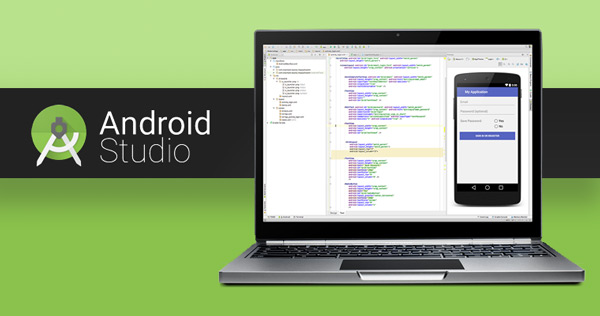
\includegraphics[width=0.7\columnwidth]{androidStudio.jpg}
	\caption{Android Studio}
	\label{fig:ejemplo}
\end{figure}

Para instalar Android Studio es necesario disponer del Java Development Kit 
(JDK) \cite{URL::JDKInfo}. 

Una vez completada la instalación del JDK, se procede a la descarga del 
AndroidStudio \cite{URL::AndroidStudio}, del SDK de Android
\cite{URL::InstallSDK} y de todos los paquetes del SDK \cite{URL::SDKPackages} 
necesarios para asegurar la compatibilidad con los dispositivos Android en
los que se desee desarrollar.
\newpage
\subsection{Atom}
\textit{Atom} \cite{URL::Atom} es un editor de texto moderno desarrollado por Github para los sistemas operativos Windows, Linux y OS X. Soporta control de versiones y 
se puede personalizar añadiendo multitud de plug-ins escritos en Node.js

\begin{figure}[h]
	\centering
	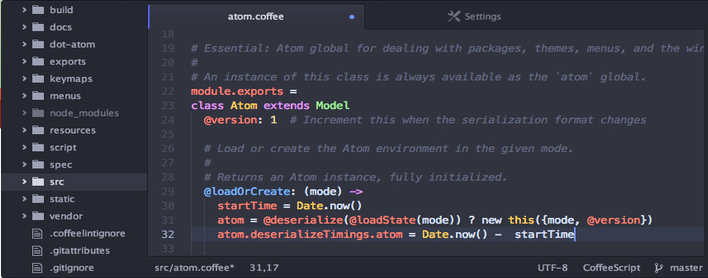
\includegraphics[width=1.0\columnwidth]{atom.png}
	\caption{Atom}
	\label{fig:ejemplo}
\end{figure}

\subsection{LaTeX y ShareLaTeX}

\textit{LaTeX} \cite{URL::LaTeX} es un sistema de composición de textos, orientado a la creación de documentos escritos que presenten una alta calidad tipográfica. 
Por sus características y posibilidades, es usado de forma especialmente intensa en la generación de artículos y libros científicos que incluyen, 
entre otros elementos, expresiones matemáticas.

\textit{ShareLaTeX} \cite{URL::ShareLatex} es un editor de LaTeX online colaborativo en tiempo real y de código libre. Y cuenta tanto con versión web como con versión de escritorio.
\newpage
\begin{figure}[h]
	\centering
	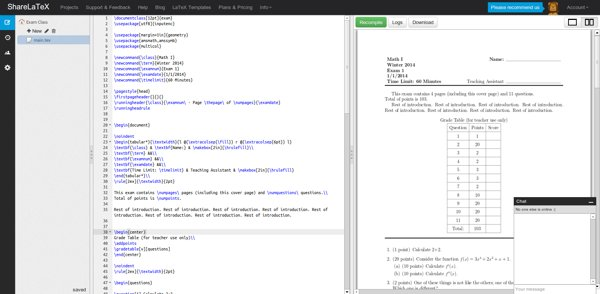
\includegraphics[width=1.0\columnwidth]{sharelatex.jpg}
	\caption{ShareLaTeX}
	\label{fig:ejemplo}
\end{figure}
\subsection{Github}
\textit{Github} \cite{URL::Github} es una plataforma de desarrollo colaborativo que sirve como repositorio de proyectos. 
Github trabaja con el sistema de control de versiones git y el código de los realizadas es almacenado 
de manera pública anunque existe también la manera de hacerlo de forma privada. 

Entre las características de esta herramienta podemos destacar:
\begin{itemize}
\item Posibilidad de tener una wiki para cada proyecto.
\item Posibilidad de tener una página web para cada proyecto.
\item Estadísticas en relación a los commits de los desarrolladores. Frecuencia, contribución y 
presentación visual de las distintas ramas del proyecto
\end{itemize}
Además la herramienta se asemeja a una red social dado que permite a cualquiera: seguir los cambios, valorar y 
ayudar a desarrollar en el proyecto.

\section{Tecnologías}
En esta sección se explicarán las tecnologías utilizadas.

\section{Sistema operativo Android}

\textit{Android} \cite{URL::Android} es un sistema operativo basado en el núcleo Linux. Fue diseñado principalmente para dispositivos 
móviles con pantalla táctil, como teléfonos inteligentes, tablets, relojes inteligentes, 
televisores y automóviles. Inicialmente fue desarrollado por Android Inc. hasta que en 2005 Google 
la compró.

Entre las características del sistema operativo se encuentran:

\begin{itemize}
\item Sevicio de mensajería, Bluetoot, videollamada etc.
\item Navegador web.
\item Multitarea.
\item Soporte para cámaras de fotos, de vídeo, pantallas táctiles, GPS, acelerómetros, 
giroscopios, magnetómetros, sensores de proximidad y de presión, sensores de luz, gamepad, 
termómetro, aceleración por GPU 2D y 3D.
\item Incluye un emulador de dispositivos, herramientas para depuración de memoria y análisis del rendimiento del software.
\item Soporte nativo para pantallas capacitivas con soporte multi-táctil.
\item Búsqueda por Google mediante voz.
\item Soporta tethering, que permite al teléfono ser usado como un punto de acceso alámbrico o inalámbrico.
\end{itemize}

\section{Django}

\textit{Django} \cite{URL::Django} es un framework web de código abierto escrito en \textit{Python} \cite{URL::Python} que sigue el patrón Modelo-Vista-Controlador. 
\newline

La meta fundamental de Django es facilitar la creación de sitios web complejos. 
Django pone énfasis en el re-uso, la conectividad y extensibilidad de componentes, el desarrollo rápido y 
el principio 'No te repitas' (DRY, del inglés Don't Repeat Yourself). Python es usado en todas las partes del 
framework, incluso en configuraciones, archivos, y en los modelos de datos.
\newline

Django necesita Python 2.5 o superior. Tiene soporte para bases de datos (PostgreSQL, MySQL y SQLite 3) y soporte de servidores web, sobretodo 
para hacer pruebas y trabajar en la etapa de desarrollo, en fase de producción se recomienda el uso de Apache.


\begin{figure}[h]
	\centering
	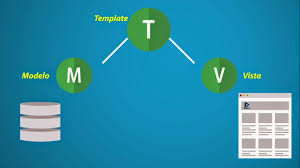
\includegraphics[width=0.5\columnwidth]{django.jpg}
	\caption{Arquitectura de Django}
	\label{fig:ejemplo}
\end{figure}


%
% ---------------------------------------------------
%
% Trabajo Fin de Grado:
% Author: Víctor Hernández Pérez 
% Correo: alu0100697032@ull.edu.es
% Capítulo: Descripción de la App
%
% ----------------------------------------------------
%

\cleardoublepage

\chapter{Descripción de la aplicación}

\section{Introducción}

\App{} es una aplicación para dispositivos Android (App) que permite ...

\subsection{Subsección}

\begin{figure}[h]
	\centering
	
\includegraphics[width=0.3\columnwidth]{cc.png}
	\caption{Imagen de ejemplo}
	\label{fig:ejemplo}
\end{figure}

%%%%%%%%%%%%%%%%%%%%%%%%%%%%%%%%%%%%%%%%
\section{Actividades}

Actividades

%
% ---------------------------------------------------
%
% Trabajo Fin de Grado:
% Author: Víctor Hernández Pérez 
% Correo: alu0100697032@ull.edu.es
% Capítulo: Desarrollo
%
% ----------------------------------------------------
%
\chapter{Desarrollo} \label{chap:Desarrollo}  

No es objeto de esta memoría explicar exhaustivamente cada una de las clases y métodos que componen \App{}.
En este capítulo se describe la implementación de las \textit{Activities} y clases más relevantes de la aplicación. 

\section{Clase \textit{Ejemplo}}

Cada instancia de la clase \textit{Ejemplo} ...

\lstinputlisting[float, language=xml, caption={Clase Ejemplo}, label={code:ejemplo}]
{listings/ejemplo.java} %% LISTING

%
% ---------------------------------------------------
%
% Trabajo Fin de Grado:
% Author: Víctor Hernández Pérez 
% Correo: alu0100697032@ull.edu.es
% Capítulo: Despliegue
%
% ----------------------------------------------------
%
\chapter{Despliegue de la aplicación}


%
% ---------------------------------------------------
%
% Trabajo Fin de Grado:
% Author: Víctor Hernández Pérez 
% Correo: alu0100697032@ull.edu.es
% Capítulo: Conclusiones y líneas futuras
%
% ----------------------------------------------------
%
\chapter{Conclusiones y líneas futuras de trabajo} \label{chap:to-do} 

Al concluir el TFG, se han adquirido los conocimientos mínimos para desarrollar aplicaciones para dispositivos Android. 
Hemos diseñado, desarrollado y desplegado una aplicación que es capaz de ...

La gestión del tiempo ha sido clave en el desarrollo, ya que se ha compaginado con la asignatura de \textit{Prácticas Externas} de cuarto curso del 
Grado en Ingeniería Informática. Gracias a ello, se ha obtenido experiencia en la gestión de tareas relacionadas con la Ingeniería del 
Software. 

También se ha trabajado en la elaboración de una memoría técnica con \textit{LaTeX}, desconocido hasta el momento. 

El desarrollo de App continuará implementando las siguientes funcionalidades:

\begin{itemize}

\item Funcionalidad 1

\item Funcionalidad 2

\end{itemize}



%
% ---------------------------------------------------
%
% Trabajo Fin de Grado:
% Author: Víctor Hernández Pérez 
% Correo: alu0100697032@ull.edu.es
% Capítulo: Summary and Conlusions
%
% ----------------------------------------------------
%
\chapter{Summary and Conlusions}
At the end of the work, I have learn some conceptsto develop Android and Django applications. The part which has more hours dedicated is the investigation of the technologies because the application has many details unknown by the author.

I have designed, developed and desployed an Android application that is able to authenticate users, access remote data and interact with a Django application which offer a reserve system to authenticated users.

Time management has been very important in this project, because it has combined with the subject ``Prácticas Externas'' also studied in the fourth year 
of the Degree in Computing Engineering. 
As a result, I have improved my skills in managing tasks related to software engineering.

I have also learned to draw up a Technical Report using \textit{LaTeX}, unknown so far.

The development of App could be continued by implementing some of the following features:
\begin{itemize}
\item Possibility of authentication against ULL servers. 
\item Improve the reserve system.
\item Add other services offer by the ULL, for example the Library.
\end{itemize}

%
% ---------------------------------------------------
%
% Trabajo Fin de Grado:
% Author: Víctor Hernández Pérez 
% Correo: alu0100697032@ull.edu.es
% Capítulo: Presupuesto
%
% ----------------------------------------------------
%
\chapter{Presupuesto}


%\newpage{\pagestyle{empty}}
%\thispagestyle{empty}

%\chapter{Presupuesto}
%\label{chapter:Presupuesto}

%\input{cap7.tex}

%%%%%%%%%%%%%%%%%%%%%%%%%%%%%%%%%%%%%%%%%%%%%%%%%%%%%%%%%%%%%%%%%%%%%%%%%%%%%%%

%%%%%%%%%%%%%%%%%%%%%%%%%%%%%%%%%%%%%%%%%%%%%%%%%%%%%%%%%%%%%%%%%%%%%%%%%%%%%%%
%\newpage{\pagestyle{empty}}
%\thispagestyle{empty}
%\begin{appendix}
%
%\chapter{Título del Apéndice 1}
%\label{appendix:1}
%\input{apendice1.tex}
%
%\chapter{Título del Apéndice 2}
%\label{appendix:2}
%\input{apendice2.tex}
%
%\end{appendix}
%%%%%%%%%%%%%%%%%%%%%%%%%%%%%%%%%%%%%%%%%%%%%%%%%%%%%%%%%%%%%%%%%%%%%%%%%%%%%%%
\addcontentsline{toc}{chapter}{Bibliografía}
\bibliographystyle{plain}
\renewcommand{\bibname}{Bibliografía}   %  Para que no aparezca Índice de figuras
\bibliography{bibliography}

%%%%%%%%%%%%%%%%%%%%%%%%%%%%%%%%%%%%%%%%%%%%%%%%%%%%%%%%%%%%%%%%%%%%%%%%%%%%%%%

\end{document}
